\documentclass[tikz,border=6pt]{standalone}
\usepackage{amsmath}
\definecolor{cG}{RGB}{31,94,165}\definecolor{cX}{RGB}{214,96,33}
\tikzset{
  vg/.style={circle,inner sep=0pt,minimum size=13pt,ball color=cG!45,draw=cG!80!black,line width=0.3pt},
  vx/.style={circle,inner sep=0pt,minimum size=13pt,ball color=cX!40,draw=cX!80!black,line width=0.3pt},
  ed/.style={line width=1.1pt,black!70},
  eb/.style={line width=0.9pt,black!45,dashed},
  ax/.style={line width=0.7pt,black!30,densely dotted},
  vl/.style={font=\small,inner sep=1pt}}
\begin{document}
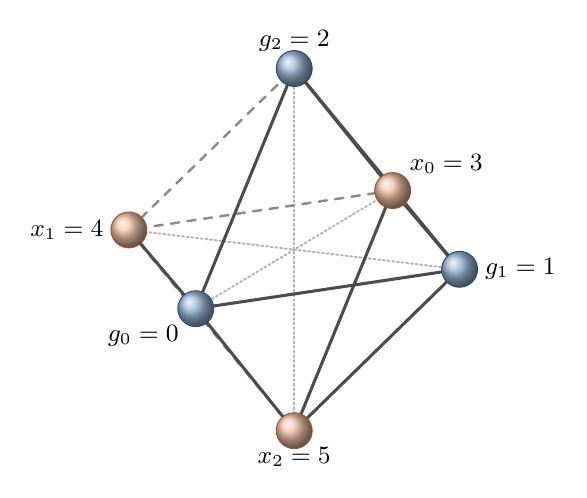
\begin{tikzpicture}[x={(-1.25cm,-0.75cm)},y={(2.1cm,-0.25cm)},z={(0cm,2.3cm)},line cap=round,line join=round]
% vertices t at +e_t and their antipodes t+3 at -e_t
\coordinate (0) at (1,0,0);  \coordinate (3) at (-1,0,0);
\coordinate (1) at (0,1,0);  \coordinate (4) at (0,-1,0);
\coordinate (2) at (0,0,1);  \coordinate (5) at (0,0,-1);
% the three antipodal pairs: the only non-adjacent pairs
\draw[ax] (0) -- (3); \draw[ax] (1) -- (4); \draw[ax] (2) -- (5);
% edges behind the front faces
\foreach \u/\v in {3/4,4/2,4/5}{\draw[eb] (\u) -- (\v);}
% visible edges
\foreach \u/\v in {0/1,1/2,2/0,0/5,5/1,0/4,1/3,3/2,3/5}{\draw[ed] (\u) -- (\v);}
\foreach \t in {0,1,2}{\node[vg] at (\t) {};}
\foreach \t in {3,4,5}{\node[vx] at (\t) {};}
\node[vl,below left=5pt] at (0) {$g_0=0$};
\node[vl,right=8pt] at (1) {$g_1=1$};
\node[vl,above=5pt] at (2) {$g_2=2$};
\node[vl,above right=5pt] at (3) {$x_0=3$};
\node[vl,left=8pt] at (4) {$x_1=4$};
\node[vl,below=5pt] at (5) {$x_2=5$};
\end{tikzpicture}
\end{document}
